\chapter{Спектральная диагностика~низкотемпературной плазмы газового разряда}
%\chapter{СПЕКТРАЛЬНАЯ ДИАГНОСТИКА НИЗКОТЕМПЕРАТУРНОЙ ПЛАЗМЫ ГАЗОВОГО РАЗРЯДА}
\label{cha:ch_1}

Плазма представляет собой ионизированное состояние вещества. Процессы
ионизации и рекомбинации в плазменном объеме сопровождаются заселением
возбужденных состояний атомных частиц и их последующим высвечиванием.
Таким образом, практически всегда плазма “светится” в широком диапазоне длин
волн. Излучение плазмы несет в себе много ценной информации о ее параметрах.

Существует целый ряд различных методов оптической спектральной
диагностики плазмы: эмиссионные и абсорбционные, лазерной индуцированной
флуоресценции (ЛИФ), рассеяния лазерного излучения на заряженных частицах,
спектроскопии высокого разрешения. Данные методы (или комбинации методов)
позволяют получить информацию о химическом составе плазмы, концентрации
метастабильных и короткоживущих возбужденных атомных частиц, концентрации
и температуре электронов и ионов. Выбор конкретных методик обуславливается
поставленными задачами и имеющейся аппаратурой.

\section{Спектральная диагностика пылевой плазмы (обзор)}
Введение пылевых частиц в плазму газового разряда влияет на спектр излучения плазмы как
непосредственно, например, уширяет спектральные линии в электрическом поле заряженных частиц,
так и опосредственно – через изменение конфигурации электрического разряда в присутствии пылевых частиц.
Пылевые частицы вносят дополнительные потери плазмы, а разряд в зависимости от режима питания компенсирует
эти потери путем изменения режима разряда. Уширение спектральных линий в сильных
электрических полях заряженных пылевых частиц исследовалось теоретически~\cite{TRINITI} и экспериментально
с помощью интерферометра Фабри-Перо~\cite{Pikalev2014}.
В теоретической работе~\cite{TRINITI} было показано, что для получения заметного эффекта уширения спектральной линии
$H_{\beta}$ необходимы совершенно фантастические концентрации пылевых частиц $N_d \sim 10^6$~см$^{-3}$ и величины
их зарядов $Q_d = 2 \cdot 10^4$~$e$.
Реальные же плазменно-пылевые структуры имеют $N_d \sim 4 \cdot 10^4$~см$^{-3}$ и $Q_d \sim 5 \cdot 10^3$~$e$~\cite{Zobnin2018}.
Что касается экспериментальной работы~\cite{Pikalev2014}, то влияния пылевых частиц на ширину спектральных линий
в пределах точности эксперимента установить не удалось.

Имеется ряд работ по экспериментальному исследованию влияния пылевого облака на электронную температуру в
высокочастотном (ВЧ) разряде~\cite{Samsonov1999}. С помощью видеокамер была построена аппроксимационная калибровка
оптической интенсивности с учетом нелинейного отклика видеокамер, а затем попиксельно выстроены искусственные
цветовые схемы. Было замечено, что электронная температура и концентрация электронов после внесения пылевых частиц стали выше.
В работе наших коллег из Германии~\cite{Mitic2009} с помощью абcорбционных методов также наблюдается увеличение
электронной температуры и концентрации электронов в ВЧ разряде. Были проведены экспериментальные и расчетные оценки.

Также совсем недавно были проведены лабораторные исследования~\cite{Pikalev2018}~и~\cite{Kostenko} интенсивностей спектральных линий
в стратифицированном разряде. Сильная неоднородность параметров плазмы в стратифицированном разряде затрудняет интерпретацию
экспериментальных результатов, поскольку конфигурации облака на границе и в объеме страты отличаются.
Для уверенности необходим эксперимент для проверки независимости описанного спектрального эффекта относительно положения облака в стратах.
Также, в данных работах лишь говорится о влиянии на электронную температуру, но никто
не связывает (даже оценочно) отношения интенсивностей с электронной температурой, отчасти это связано с математическими
трудностями решения кинетического уравнения Больцмана в земных условиях с учетом страт.
Более того, в работе~\cite{Pikalev2018} эффект влияния пылевого облака на
интенсивность спектральных линий для $Ne$ и $Ar$ примерно равен погрешностям измерения.

\section{Кинетика заселения возбужденных атомных состояний в плазме}
\label{sec:kinetika}
Для диагностики изменения электронной температуры $T_e$ по изменению
интенсивности спектральных линий необходимо построить модель заселения уровней
неона в зависимости от электронной температуры. Вид эмиссионного спектра
излучения положительного столба газового разряда в неоне определяется
структурой энергетических уровней атома неона и кинетикой их заселения и
расселения. При относительно высоких давлениях плазмы (более 1~атмосферы) заселенность
возбужденных уровней атомов неона описывается равновесным больцмановским
распределением:
\begin{equation}
    N_i(\epsilon) = N_0 e^{- {\epsilon \over T_e}},
\end{equation}
где $N_i$~--~населенность возбужденного уровня $i$, $N_0$~--~населенность основного уровня,
электронная температура $T_e$ равна ионной температуре $T_i$ и температуре
нейтральных атомов $T_n$. При понижении давления плазмы все три температуры всё
больше различаются друг от друга, а заселенность возбужденных уровней
отклоняется от равновесного больцмановского. При тлеющем разряде распределение населенностей атомных уровней по
энергиям всегда является неравновесным и требует для своего описания детальную
кинетическую радиационно-столкновительную (РС) модель.

Рассмотрим схему энергетических уровней атома неона, приведенную на
рисунке \ref{fig:energy_diag_NE}. Основное энергетическое состояние атома неона представляет собой
полностью заполненные электронные оболочки $1s$, $2s$ и $2p$ и, соответственно,
характеризуется полным орбитальным моментом $L = 0$ и спиновым моментом $S = 0$, а
терм основного состояния обозначается как $^1S_0$. Первыми возбужденными
состояниями является $1s$-группа (обозначения Пашена) из 4-х~уровней в диапазоне
энергий от 16.6 до 16.8 эВ.
Далее по возрастанию энергии следует $1p$-группа из 10~уровней в в диапазоне
энергий от 18.4 до 19.0 эВ. Доступными для диагностики населенностей по спонтанному
излучению плазмы являются группа $2p$-уровней и некоторые уровни из $3d$-группы.

\begin{figure}[t]
  \centering
  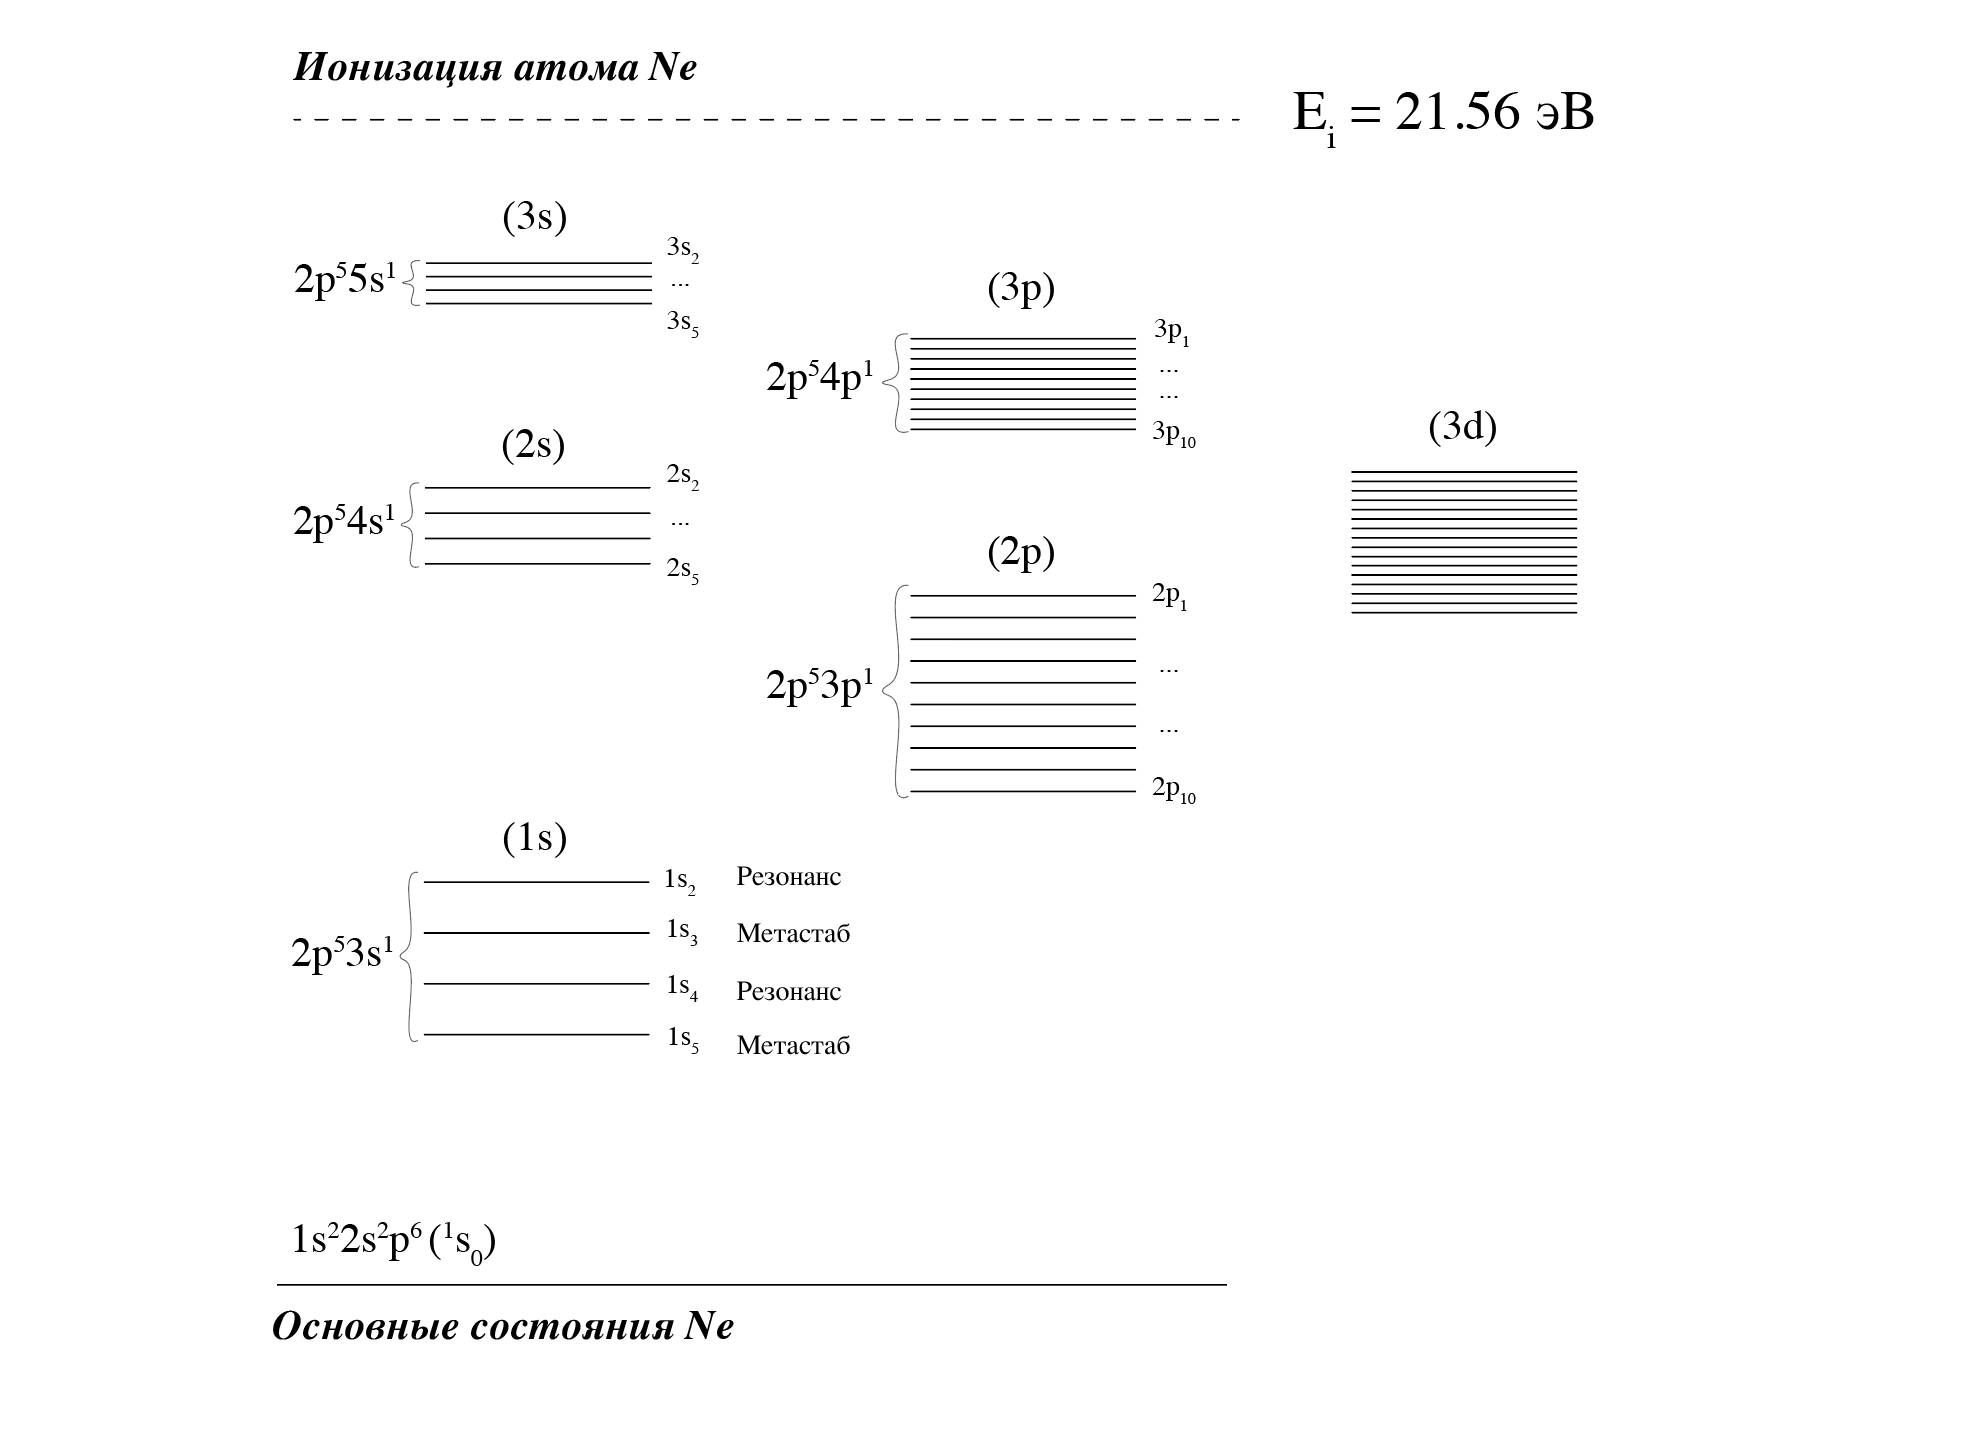
\includegraphics[width=16cm]{figures/energy_diag_NE}
  \caption{Схематичная диаграмма энергетических состояний атома неона и их обозначения в термах Пашена}
  \label{fig:energy_diag_NE}
\end{figure}

Спектры излучения газоразрядной плазмы определяются населенностью $N_j$ соответствующих возбужденных атомных уровней $E_j$.
Тогда интенсивность соответствующей атомной спектральной линии составит:
\begin{equation}
    I_{j,i} = A_{j,i}h\nu_{j,i}⋅N_j,
\end{equation}
где $A_{j,i}$  - коэффициент Эйнштейна для перехода $j → i$, $N_j$ - населенность возбужденного уровня $j$.
Задача спектральной диагностики плазмы сводится к построению теоретических моделей, связывающих
параметры плазмы (в первую очередь, концентрации электронов $n_e$ и их температуру $T_e$) с интенсивностями спектральных
линий $I_{j,i}$. Выбор той или иной модели зависит от параметров плазмы: ее химического состава, плотности,
степени ионизации и равновесности.

%\begin{figure}[t]
%    \begin{center}
%         \subfloat[\label{sub:fig11a}]{
%           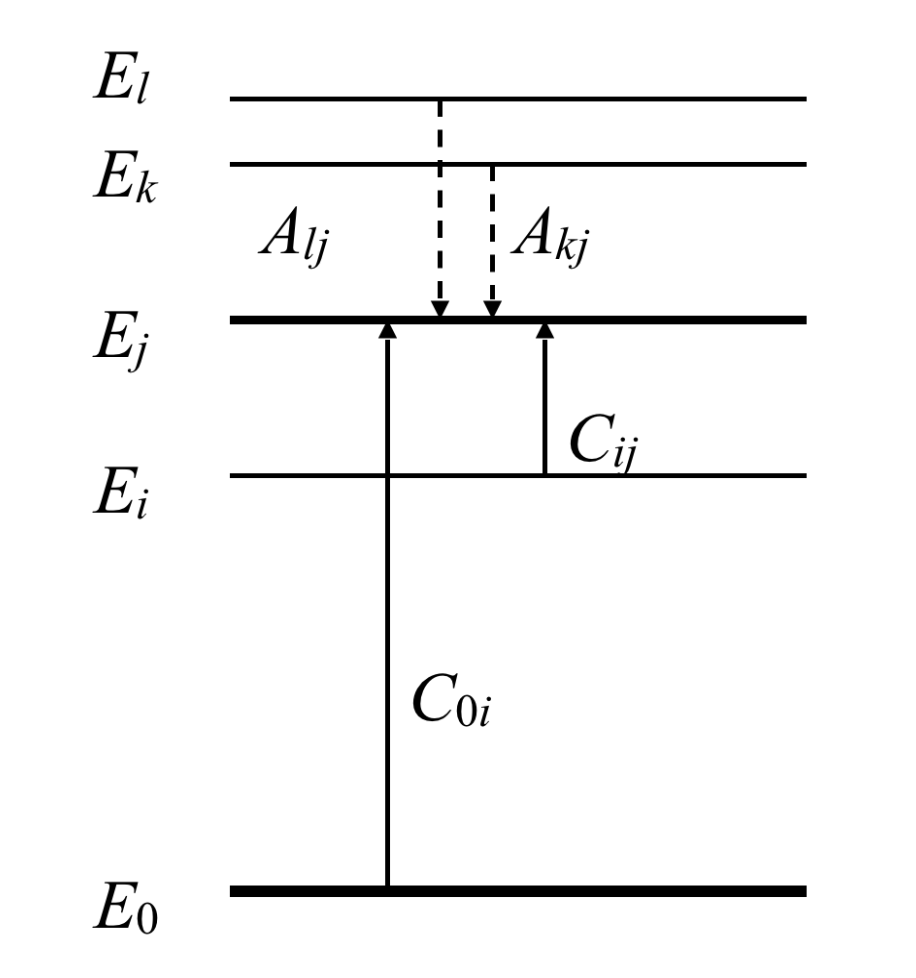
\includegraphics[width=0.35\textwidth]{figures/fig11a}
%         }
%         \hspace{0.05\columnwidth}
%         \subfloat[\label{sub:fig11b}]{
%           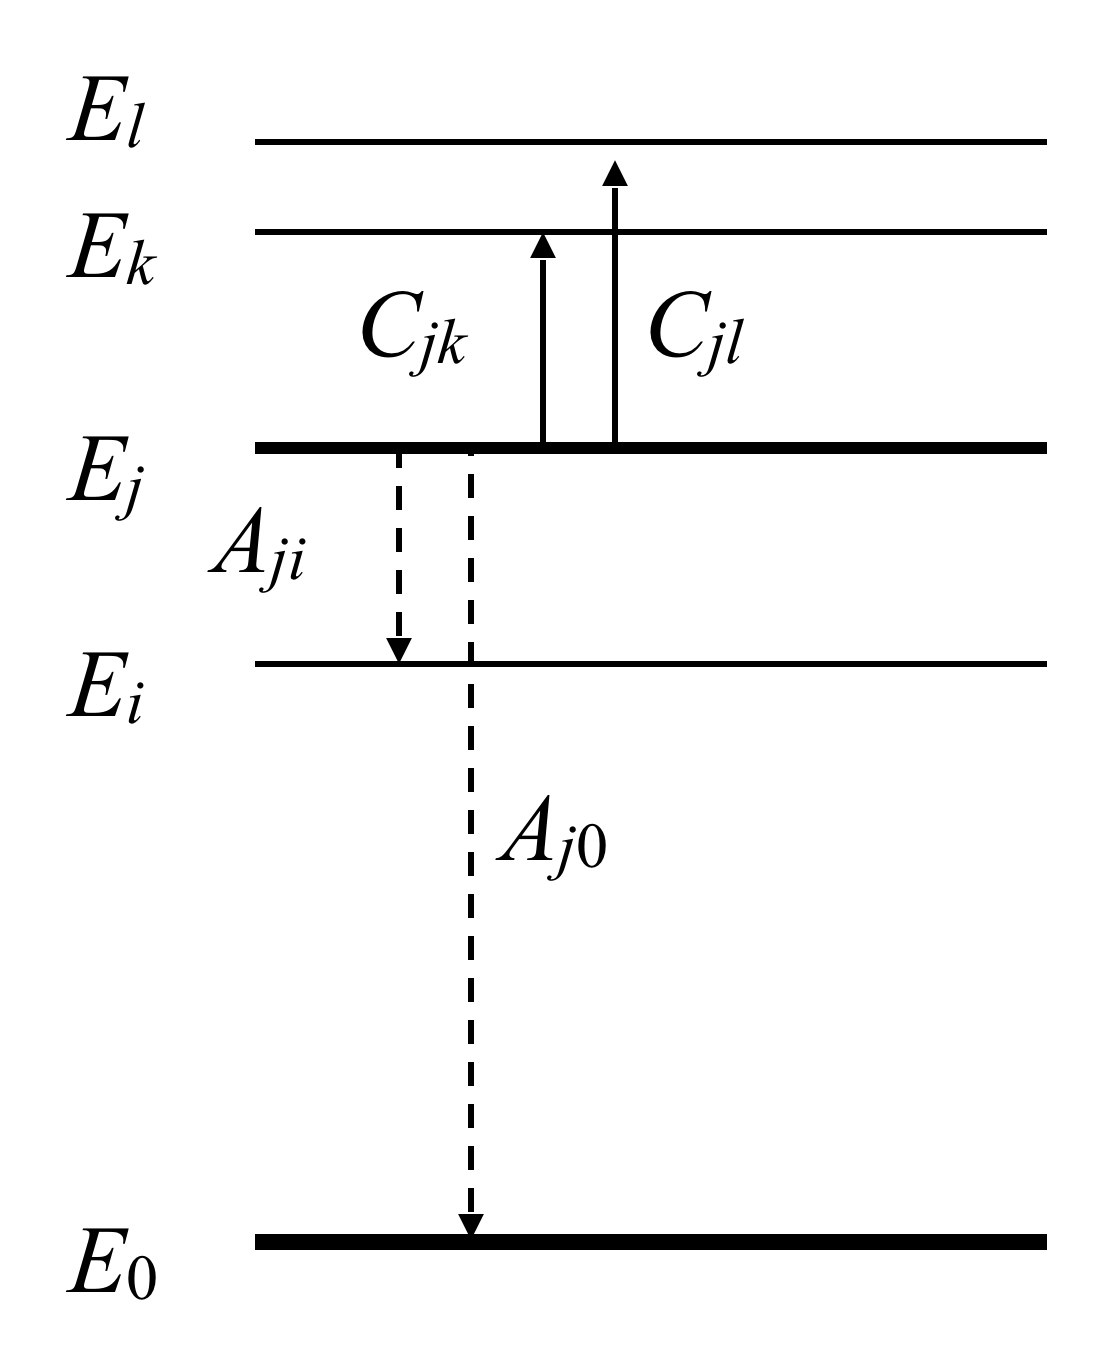
\includegraphics[width=0.305\textwidth]{figures/fig11b}
%         }
%         \caption{Схема основных процессов уровня: \pt(а) заселение, \pt(б) расселение.}
%         \label{fig:fig11}
%    \end{center}
%\end{figure}
Населенность $N_j$ уровня $E_j$ в стационарном случае определяется балансом процессов его заселения
и расселения. Схема основных процессов заселения уровней $Ne$ представлена на рисунке~\ref{fig:energy_diag_NE}.
Основным процессом заселения уровней является заселение прямым
электронным переходом с основного состояния $E_0$, а также, в меньшей мере с метастабильных состояний. Последние
для упрощения расчетной модели можно не учитывать, поскольку концентрация электронов в метастабилях мала по сравнению
с концентрацией в основном состоянии~\cite{Zobnin2014}.
\begin{figure}[t]
  \centering
  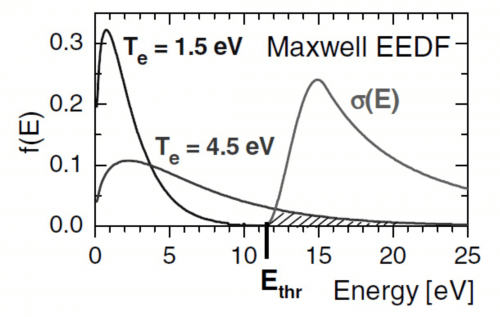
\includegraphics[width=8cm]{figures/fig12}
  \caption{Типичный вид сечения \math{\sigma}$ и максвелловской ФРЭЭ. \math{T_e}$ - температура электронов, \math{E_{thr}}$ - пороговая энергия.}
  \label{fig:fig12}
\end{figure}
Скоростные коэффициенты процессов $X_{0,j}$ и $X_{i,j}$ определяются соотношениями:
\begin{equation}
    X_{0,j} = \sqrt{2 \over m_e} \int_{E_j}^{\infty} \sigma_{0,j}(\epsilon) f(\epsilon) \epsilon d\epsilon,
    \label{eq:X_0j}
\end{equation}
и
\begin{equation}
    X_{i,j} = \sqrt{2 \over m_e} \int_{E_j - E_i}^{\infty} \sigma_{i,j}(\epsilon) f(\epsilon) \epsilon d\epsilon,
\end{equation}
соответственно, где $\sigma_{0,j}$~--~сечение возбуждения из основного состояния в состояние $j$,
$\sigma_{i,j}$~--~сечение возбуждения из состояния $i$ в состояние $j$, $m_e$~--~масса электрона, $f(\epsilon)$~--~функция
распределения электронов по энергиям (ФРЭЭ). Расчетные и экспериментальные сечения возбуждения $\sigma_{0,j}(E)$ и
$\sigma_{i,j}(E)$ можно найти в литературе или в базе данных NIST \cite{NIST}.
Типичный вид сечений представлен на рисунке \ref{fig:fig12}. Что касается вида ФРЭЭ, то она сильно зависит от параметров плазмы.
При высоких давлениях ФРЭЭ приближается к максвелловской функции. Однако, при низких давлениях плазма сильно неравновесна, и вид функции ФРЭЭ должен
быть определен дополнительными методами. Кроме столкновительного заселения уровень $E_j$ заселяется
также путем радиационного распада верхних $k$-уровней $E_k~>~E_j$ cо скоростью $A_{kj}$ при $k > j$, но в рамках данной задачи
предлагается пренебречь этими процессами в силу низкой концентрации.

Приравняв скорости заселения и расселения для выбранного уровня \math{E_j}$, мы получим уравнение относительно ФРЭЭ \math{f(\epsilon)}$.
Для решения данного уравнения необходимы дополнительные данные о виде ФРЭЭ.
Эти данные могут быть получены путем решения кинетического уравнения Больцмана для соответствующих условий.

\section{Уравнение Больцмана для функции распределения электронов по энергиям в положительном столбе газового разряда постоянного тока.}

Газовые разряды представляют собой крайне неравновесную систему, в которой средняя энергия электронов (температура)
на два порядка превышает температуру газа. ФРЭЭ формируется в результате нагрева
электронов электромагнитными полями и столкновениями их с нейтральными атомами, почти во всех случаях это распределение
отклоняется от равновесного (максвелловского). Решение кинетического уравнения Больцмана для ФРЭЭ является
важнейшей задачей для точного моделирования плазмы, так как многие явления невозможно правильно понять
без кинетического анализа. Уравнение Больцмана существенно можно упростить из-за большого различия масс электронов и атомов.
В силу данного различия, затухание энергии электронов в упругих столкновениях с атомами происходит гораздо медленнее,
чем затухание импульса электронов (\math{m_e \ll M_a}$). Как следствие, функция распределения электроном в скоростном пространстве (ФРЭС) может быть представлена как сумма
большой изотропной \math{f_0}$ и малой анизотропной частей \math{f_1}$.

Выделяют 3 существенно различных случая. Первый случай, когда величины \math{P L \gg 1}$ и \math{{E P} \ll 1}$, где
\math{P}$ - давление газа, \math{L}$ - характерный размер плазмы, \math{E}$ - электрическое поле, а
пространственные градиенты \math{f_0}$ и \math{f_1}$ малы и определены локальными значениями электрического поля,
электронной плотности и составом плазмы. Тогда электроны могут быть описаны уравнениями жидкости с коэффициентами переноса,
полученными из локальной (не максвелловской) ФРЭС. Обычно через уравнение Больцмана решают задачу нахождения
коэффициентов переноса и скоростей протекания реакции для данного приближения.

Второй случай соответствует столкновительной плазме, где характерный размер плазмы \math{L}$ значительно больше средней длины
свободного пробега электронов \math{\lambda}$, но сравним с длиной релаксации энергии электрона \math{\lambda_\epsilon}$.
В этом нелокальном режиме изотропная часть ФРЭС \math{f_0}$ в заданной точке зависит не только от электрических полей в этой точке,
но и от свойств плазмы в окрестности точки размера (эффект памяти), а анизотропная часть \math{f_1}$ является лишь функцией
электрического поля \math{E}$. В этом столкновительном режиме плазма не может быть описана гидродинамикой.

В третьем случае, при дальнейшем уменьшении \math{P L}$, средняя длина свободного пробега электрона будет сравнима c характерным размером плазмы
(\math{\lambda \sim L)$. В этом почти бесстолкновительном случае анизотропная часть в точке определяется не только
значением напряженности электрического поля в этой точке, но и профилем электрического поля вдоль траектории электрона.
В результате локальная зависимость между плотностью тока и электрическим полем (закон Ома) становится недействительной \cite{Kolobov}.

Плазма тлеющего разряда низкого давления имеет сильно неравновесный характер. Рождение заряженных частиц происходит
преимущественно в объемных процессах, а гибель на стенках разрядной камеры. Энергию электроны приобретают,
разгоняясь в электрическом поле, а теряют в упругих и неупругих столкновениях. Количественное описание этих процессов
возможно только на кинетическом уровне \cite{Zobnin2009}. В данной работе положительный столб газового разряда находится
под низким давлением порядка 60~Па и имеет диаметр трубки 30~мм (см. раздел \ref{sec:sec_31}),
а значит для описания кинетических процессов с помощью уравнения Больцмана необходимо пользоваться почти бесстолкновительным приближением.

Кинетическое уравнение Больцмана представляет собой интегродифференциальное уравнение, описывающее эволюцию функции
распределения частиц в шестимерном (6-D) фазовом пространстве. Данное уравнение было выведено Людвигом Больцманом в 1872 г.
Оно до сих пор остается основой кинетической теории газов и оказывается плодотворным не только для исследования
классических газов, которые имел в виду Больцман, но - при соответствующем обращении - и для излучения переноса
электронов в твердых телах и плазме \cite{Cherchin'yani}. В общем виде оно выглядит следующим образом (также данное
уравнение называют уравнением Власова):

\begin{equation}
    {\partial f_e \over \partial t} + (\vec{v}, \vec{\Delta}_r) f_e + (\vec{a}, \vec{\Delta}_v) f_e = I,
    \label{eq:vlasov}
\end{equation}
где \math{f_e = f_e(\vec{r}, \vec{v}, t)}$~--~функция распределения электронов по скоростям,
\math{\vec{r}}$~--~вектор положения в физическом пространстве, \math{\vec{v}}$~--~вектор скорости,
\math{\vec{a}}$~--~вектор ускорения, \math{t}$~--~время, \math{I}$~--~интеграл столкновений,
является интегральным оператором в пространстве скоростей, в котором должны быть учтены все элементарные процессы
с участием электронов, приводящие к изменению их числа в объеме \math{dx dy dz dv_x dv_y dv_z}$ фазового пространства.

Решение этого интегродифференциального нелинейного уравнения сопряжено с огромными математическими трудностями и
поэтому всегда проводится с привлечением ряда серьезных упрощений. Многие сотни журнальных публикаций посвящены
конкретным расчетам \math{f(V)}$ в различных условиях, однако среди них далеко не всегда удается найти требуемое.
Вместе с тем экспериментатору часто приходится хотя бы оценить ожидаемый вид \math{f(V)}$ в условиях его работы \cite{Kolesnikov}.

%{e \over m_e} \vec{E}

Для слабоионизированной плазмы столкновения электронов с нейтралами обычно преобладают над столкновениями между
заряженными частицами. Из-за разницы масс электрона и атома (\math{m_e \ll M_a}$) интеграл столкновения
для упругих взаимодействий электронов с тяжелыми нейтралами может быть записан в так называемой форме Лоренцевского газа
\cite{Kolobov}:
\begin{equation}
    I_{el} = - {1 \over v^2} {\partial \over \partial v} v^2 \Gamma - N v \int_{S^2} \sigma (v, |\Omega - \Omega^{'}|) [f(v, \Omega^{'}) - f(v, \Omega)] d \Omega,
    \label{eq:lorentz}
\end{equation}
где \math{\Omega}$~--~телесный угол фазового пространства скоростей на единичной сфере \math{S^2}$ (\math{\vec{v} = v \Omega}$),
\math{\sigma}$~--~сечение столкновения, \math{N}$~--~концентрация атомов газа, поток \math{\Gamma}$ задается следующим образом:
\begin{equation}
    \Gamma = - {\delta \nu \over 2} \big{(} v f + {T \over m} {\partial f \over \partial v} \big{)},
\end{equation}
где \math{T}$~--~температура газа, \math{\nu}$~--~транспортная частота столкновений и \math{\delta = (2m / M)}$~--~
средняя доля энергии, которая теряется электронами в упругих столкновений. Первое слагаемое в (\ref{eq:lorentz}) мало, оно
отвечает за обмен энергиями между электронами и нейтралами. Второе слагаемое в (\ref{eq:lorentz}) описывает столкновения
электронов с бесконечно тяжелыми частицами, которые в основном не меняют свою энергию, а лишь изотропно меняют
распределение электронов. Таким образом для того, чтобы ФРЭС пришла в равновесие с полем необходимо, чтобы прошло время
намного превышающе \math{({\nu m / M})^{-1}}$ \cite{Tsendin}.

Таким образом, для почти бесстолкновительного случая в качестве приближения ФРЭС для решения уравнения Власова (\ref{eq:vlasov}) можно
использовать двухчленное приближение:
\begin{equation}
    f_e(\vec{r}, \vec{v}, t) = f_0(\vec{r}, \vec{v}, t) + { \vec{v} \over v} \vec{f_1} (\vec{r}, \vec{v}, t),
\end{equation}
где \math{f_1}$ отвечает за анизотропию.

Подставив это приближение в уравнение (\ref{eq:vlasov}) и усреднив по направлениям скоростей (в силу их изотропности из-за
столкновений с тяжелыми частицами), получим следующую систему уравнений, которую называют системой
Давыдова-Эллиса \cite{Kolobov}:
\begin{equation}
 \begin{cases}
  {\partial \vec{f_1} \over \partial t} + \nu \vec{f_1} = - v \nabla f_0 - {e \vec{E} \over m} {\partial f_0 \over \partial v}
   \\
   {\partial f_0 \over \partial t} + {v \over 3} div(\vec{f_1}) + {1 \over 3v^2} {\partial \over \partial v } ({ v^2 e \vec{E} \over m} \vec{f_1} ) = S_0
 \end{cases},
 \label{eq:davydov-ellis}
\end{equation}
здесь \math{e}$~--~модуль заряда электрона, \math{m}$~--~масса электрона, \math{S_0}$ —  часть интеграла столкновений,
отвечающая за упругие и неупругие электрон-атомные столкновения и электрон-электронные взаимодействия

В левой части первого уравнения системы (\ref{eq:davydov-ellis}) можно пренебречь слагаемым
{\partial \vec{f_1} \over \partial t}$, так как мы рассматриваем выход ФРЭС на стационарный уровень во времени,
где анизотропические эффекты уже не имеют значения.

Перейдя от скоростей к энергиям \math{v = \sqrt{2 \epsilon \over m}}$,
\math{{\partial f(v) \over \partial v}  = {\partial f(\epsilon) \over \partial \epsilon} \sqrt{2 \epsilon m}}$
в системе Давыдова-Эллиса (\ref{eq:davydov-ellis}) и подставив выражение для \math{\vec{f_1}}$ в нижнее уравнение, получим:
\begin{equation}
    \begin{gathered}
        \sqrt{\epsilon} {\partial f_0 \over \partial t} = \sqrt{2 \over m} \big{[} S_0 + {\partial \over \partial \epsilon}
        [\epsilon^{3 \over 2} ({2 m \over M} \nu f_0 + {e^2 (\vec{E}, \vec{E}) \over 3 \nu} {\partial f_0 \over \partial \epsilon})] \big{]}
    \end{gathered},
\end{equation}
где \math{M}$ - масса молекулы неона.

Поскольку столб газового разряда геометрически представляет собой продольную трубку,
вдоль которой течет ток, то модуль электрического поля равен продольной составляющей \math{|\vec{E}|} = E_z}$, также его
называют осевым электрическим полем. Подставив значение транспортной частоты \math{\nu = N_g \sigma_t \sqrt{\epsilon}}$ и
осевого электрического поля, а также выполнив незначительные преобразования (в том числе переобозначение \math{f_0 = f}$), получим:
\begin{equation}
    \begin{gathered}
        \sqrt{\epsilon} {\partial f \over \partial t } = \sqrt{2 \over m} \big{[} S_0 + 2 {m \over M} N_g
        {\partial \over \partial \epsilon} \big{[} \sigma_t \epsilon^2 f \big{]}
        + {e^2 E_z^2 \over 3 N_g} {\partial \over \partial \epsilon} \big{[} {\epsilon \over \sigma_t}
        {\partial f \over \partial \epsilon} \big{]} \big{]}
    \end{gathered},
    \label{eq:main_eq}
\end{equation}

Вид \math{S_0}$ зависит от того, какие взаимодействия с электронами учитываются.
В данной работе использовался следующий вид \math{S_0}$, записанный в дискретной форме:
\begin{equation}
    S_0 = \sum_k \big{[} \sqrt{\epsilon + \epsilon_k} \nu_k (\epsilon + \epsilon_k)f(\epsilon + \epsilon_k) - \sqrt{\epsilon} \nu_k(\epsilon)f(\epsilon) \big{]},
    \label{eq:S_0}
\end{equation}
суммирование проводится по всем верхним энергетическим уровням k, которые больше аргумента функции \math{\epsilon}$,
частота столкновения k-уровня записывается так \math{\nu_k(\epsilon) = \sigma_k(\epsilon)N_g\sqrt{\epsilon}}$,
\math{N_g}$ - концентрация атомов.

В почти бесстолкновительном случае для поиска концентрации атомов Ne \math{N_g}$ можно воспользоваться уравнением состояния идеального газа,
поскольку атомы между собой почти не взаимодействуют:
\begin{equation}
    N_g = {P \over k_b T},
    \label{eq:concentration}
\end{equation}
где \math{P}$~--~давление газа 60~Па; \math{k_b}$~--~постоянная Больцмана; \math{T}$~--~температура газа 294~K.

\section{Решение уравнения Больцмана и результаты}

В данном подразделе описываются численные подходы, алгоритмы и аппроксимации необходимые для нахождения численного решения
функций распределения электронов для различных осевых электрических полей в диапазоне \math{1 \le E_z \le 10}$~В/см,
которые задаются параметрически.

Рассматривается задача решения разностной схемы относительно \math{f}$ на основе уравнений (\ref{eq:main_eq}) и (\ref{eq:S_0}).
Данная задача является краевой: вероятность нахождения электронов при бесконечно большой энергии стремится к нулю, а
вероятность нахождения электронов с положительном энергией максимальна, т.е. первая производная ФРЭЭ по энергии в нуле
будет равна нулю. Имеем следующие граничные условия:
\begin{equation}
    \begin{cases}
        {d f \over d \epsilon}(0) = 0
        \\
        f(\infty) = 0
    \end{cases}.
    \label{eq:borders}
\end{equation}

Если обратить внимание на уравнения (\ref{eq:main_eq}) и (\ref{eq:S_0}), то становится ясно, что аналитически выразить
\math{f}$ для явного построения разностной схемы невозможно, поскольку в (\ref{eq:S_0}) \math{f}$ принимает значения для
аргументов, отличных от \math{\epsilon}$. Следовательно, при данной трактовки задачи необходимо получить дополнительное граничное
условие для каждого элемента суммирования \math{\epsilon_k}$, например с помощью двухточечной краевой задачи (метод стрельбы),
и сводить исходную задачу к задаче Коши. Это довольно сложный подход, более того, нет необходимости для каждого момента времени
решать задачу Коши, поскольку нас интересует ФРЭЭ при выходе на стационарный уровень во времени, а не при сложных переходных процессах.

Предполагается, что функция распределения электронов при заданном электрическом поле выйдет на стационарый уровень: из-за
невысоких полей данное предположение более, чем разумно. Поэтому будем высчитывать с помощью метода временной эволюции
относительную разницу ФРЭЭ между итерациями по времени и смотреть, если относительное изменение достаточно незначительно, то ФРЭЭ вышла
на стационарный уровень; далее решается краевая задача с граничными условиями (\ref{eq:borders}).
Построим разностную схему для данного подхода:
\begin{equation}
\begin{small}
    \begin{gathered}
        f^n(\epsilon) = f^{n-1}(\epsilon) + \Delta t \sqrt{2 \over m \cdot \epsilon}
        \Big{[} N_g \sum_k
            \big{[}
                F^{n-1}_k (\epsilon + \epsilon_k) - F^{n-1}_k (\epsilon)
            \big{]} + \\
        {2 m N_g \over M}
            \big{[}
                {F^{n-1}_t(\epsilon + \Delta \epsilon) \cdot (\epsilon + \Delta \epsilon) -
                F^{n-1}_t(\epsilon - \Delta \epsilon) \cdot (\epsilon - \Delta \epsilon)  \over 2 \Delta \epsilon }
            \big{]} + \\
        {1 \over \Delta \epsilon} \cdot {e^2 E_z^2 \over 3 N_g} \cdot
            \big{[}
                {\epsilon + { \Delta \epsilon \over 2 } \over  \sigma_t(\epsilon + { \Delta \epsilon \over 2 })} \cdot
                {f^{n-1}(\epsilon + \Delta \epsilon) - f^{n-1}(\epsilon) \over \Delta \epsilon } -
                {\epsilon - { \Delta \epsilon \over 2 } \over  \sigma_t(\epsilon - { \Delta \epsilon \over 2 })} \cdot
                {f^{n-1}(\epsilon) - f^{n-1}(\epsilon - \Delta \epsilon) \over \Delta \epsilon }
            \big{]}
        \Big{]}
    \end{gathered},
\end{small}
\label{eq:razh_scheme}
\end{equation}
где \math{\epsilon}$~--~энергия в~эВ; \math{\Delta \epsilon}$~--~шаг по энергии в~эВ;
\math{f^n (\epsilon)}$~--~ФРЭЭ с энергией \math{\epsilon}$, имеющая \math{n}$-й шаг по времени;
\math{\sigma_t (\epsilon)}$~--~транспортное сечение упругого рассеяния;
\math{\sigma_k (\epsilon)}$~--~сечение неупругих столкновений для k-уровня;
\math{N_g}$~--~концентрация атомов \math{Ne}$ в см^{-3}; \math{M}$~--~масса молекулы Ne в граммах;
\math{m}$~--~масса электрона в граммах; \math{e}$~--~заряд электрона в Кл;
\math{k}$~--~итератор суммирования по всем энергиям верхних уровней, значения которых больше \math{\epsilon}$;
\math{E_z}$~--~осевое электрическое поле, которое задается параметрически в диапазоне \math{1 \le E_z \le 10}$~В/см с шагом \math{0.1}$~В/см;
для удобства записи выполнена замена
\math{F^n_i}(\epsilon) = f^n(\epsilon) \cdot \sigma_i(\epsilon) \cdot \epsilon }$, где \math{i}$ обозначает природу сечения.

\begin{figure}[t]
  \centering
  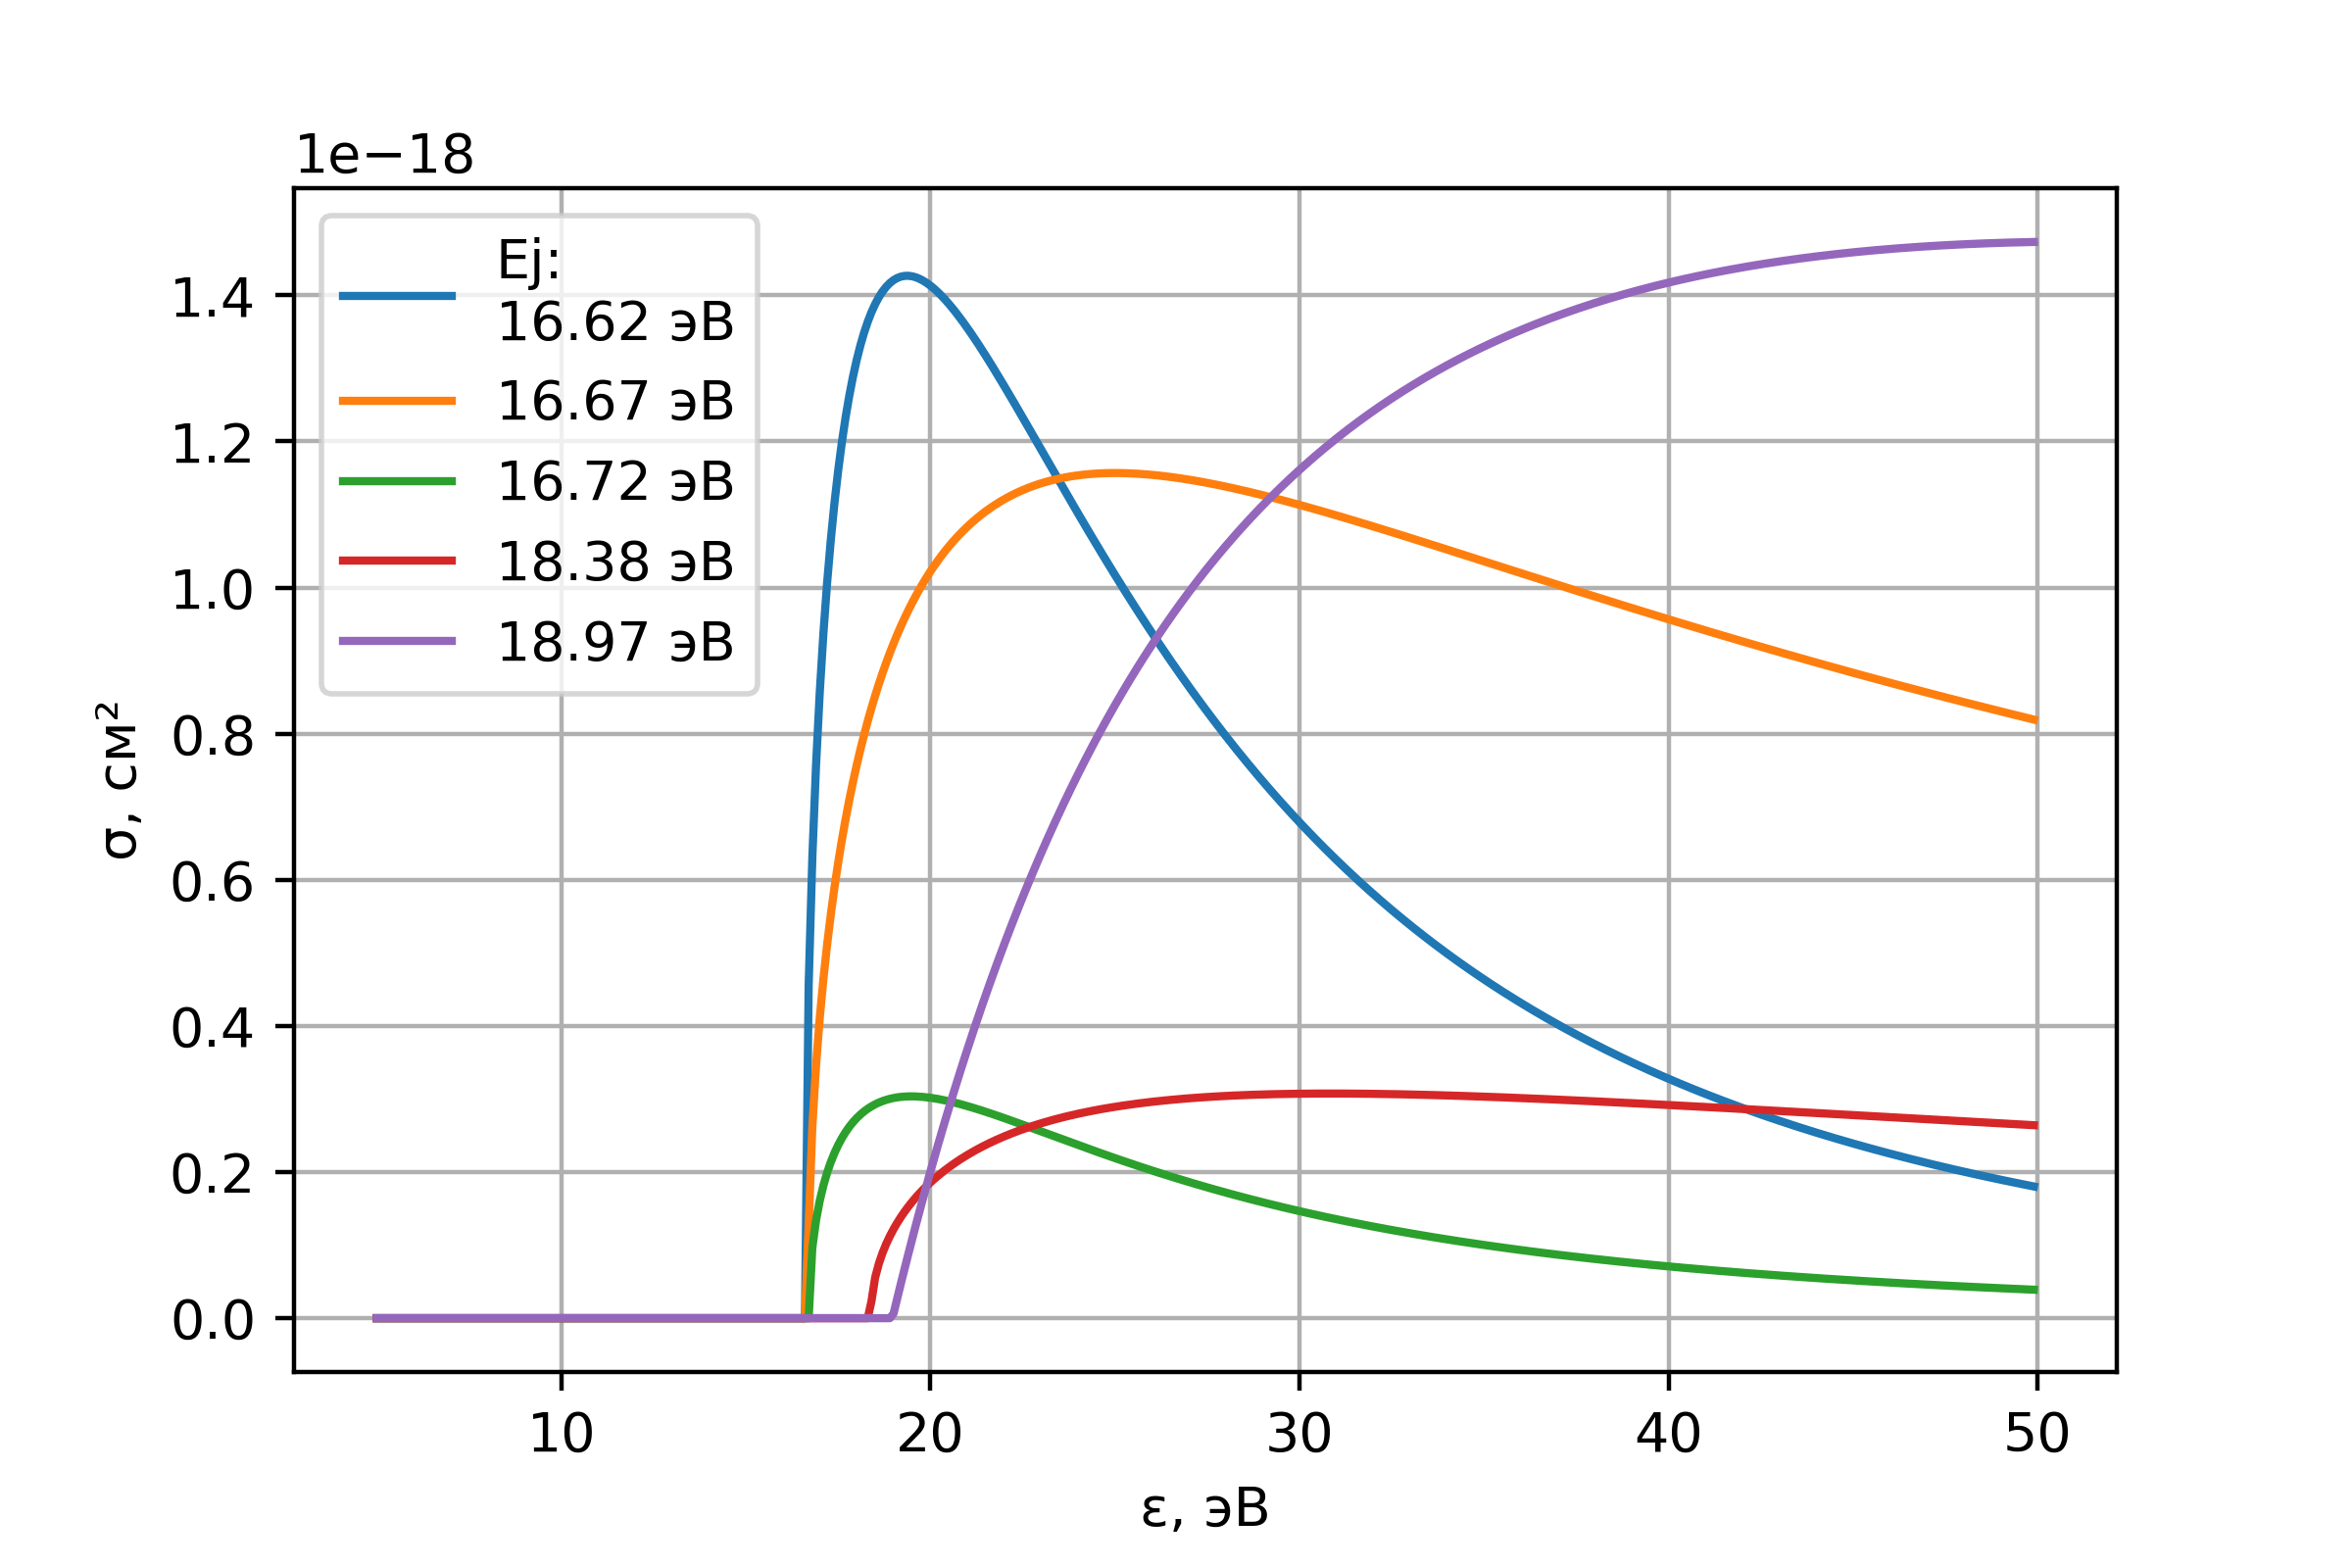
\includegraphics[width=15cm]{figures/cross_sections}
  \caption{Графическое представление некоторых аппроксимаций сечений возбуждения $\sigma_{E_j}$ для различных энергетических уровней $E_j$.}
  \label{fig:cross_sections}
\end{figure}

На языке разностной схемы граничные условия (\ref{eq:borders}) будут выглядить следующим образом:
\begin{equation}
    \begin{cases}
        f^n_0 = f^n_1
        \\
        f^{n}_K = 0
    \end{cases},
    \label{eq:razn_borders}
\end{equation}
где K~--~максимальное количество шагов по энергии, в рамках данной задачи энергию равной 50~эВ можно считать уже бесконечно большой.
То есть при шаге \math{\Delta \epsilon = 0.1}$~эВ максимальное количество шагов по энергии будет \math{K = 500}$.

В качестве начальных условий при \math{t = 0}$ для первого вычисления ФРЭЭ (при \math{E = 1}$~В/см) предлагается взять
распределение Больцмана:
\begin{equation}
    f^0 (\epsilon) = 0.7 \cdot e^{- {\epsilon \over 6}}.
    \label{eq:start_condition}
\end{equation}

Данная функция намного ближе к итоговому решению, чем прямая, а значит для сходимости нужно будет выполнить меньше итераций
по времени: чем приближеннее возьмем начальное условие, тем быстрее наступит стационарный уровень. По данным соображениям
для подсчета ФРЭЭ для следующих полей удобнее всего брать за начальные условия результаты предыдущего расчета.

В данной работе использовались следующие аналитические аппроксимации для сечений элементарных процессов \cite{Zobnin2009} и
\cite{Jung2011}:
\begin{figure}[t]
  \centering
  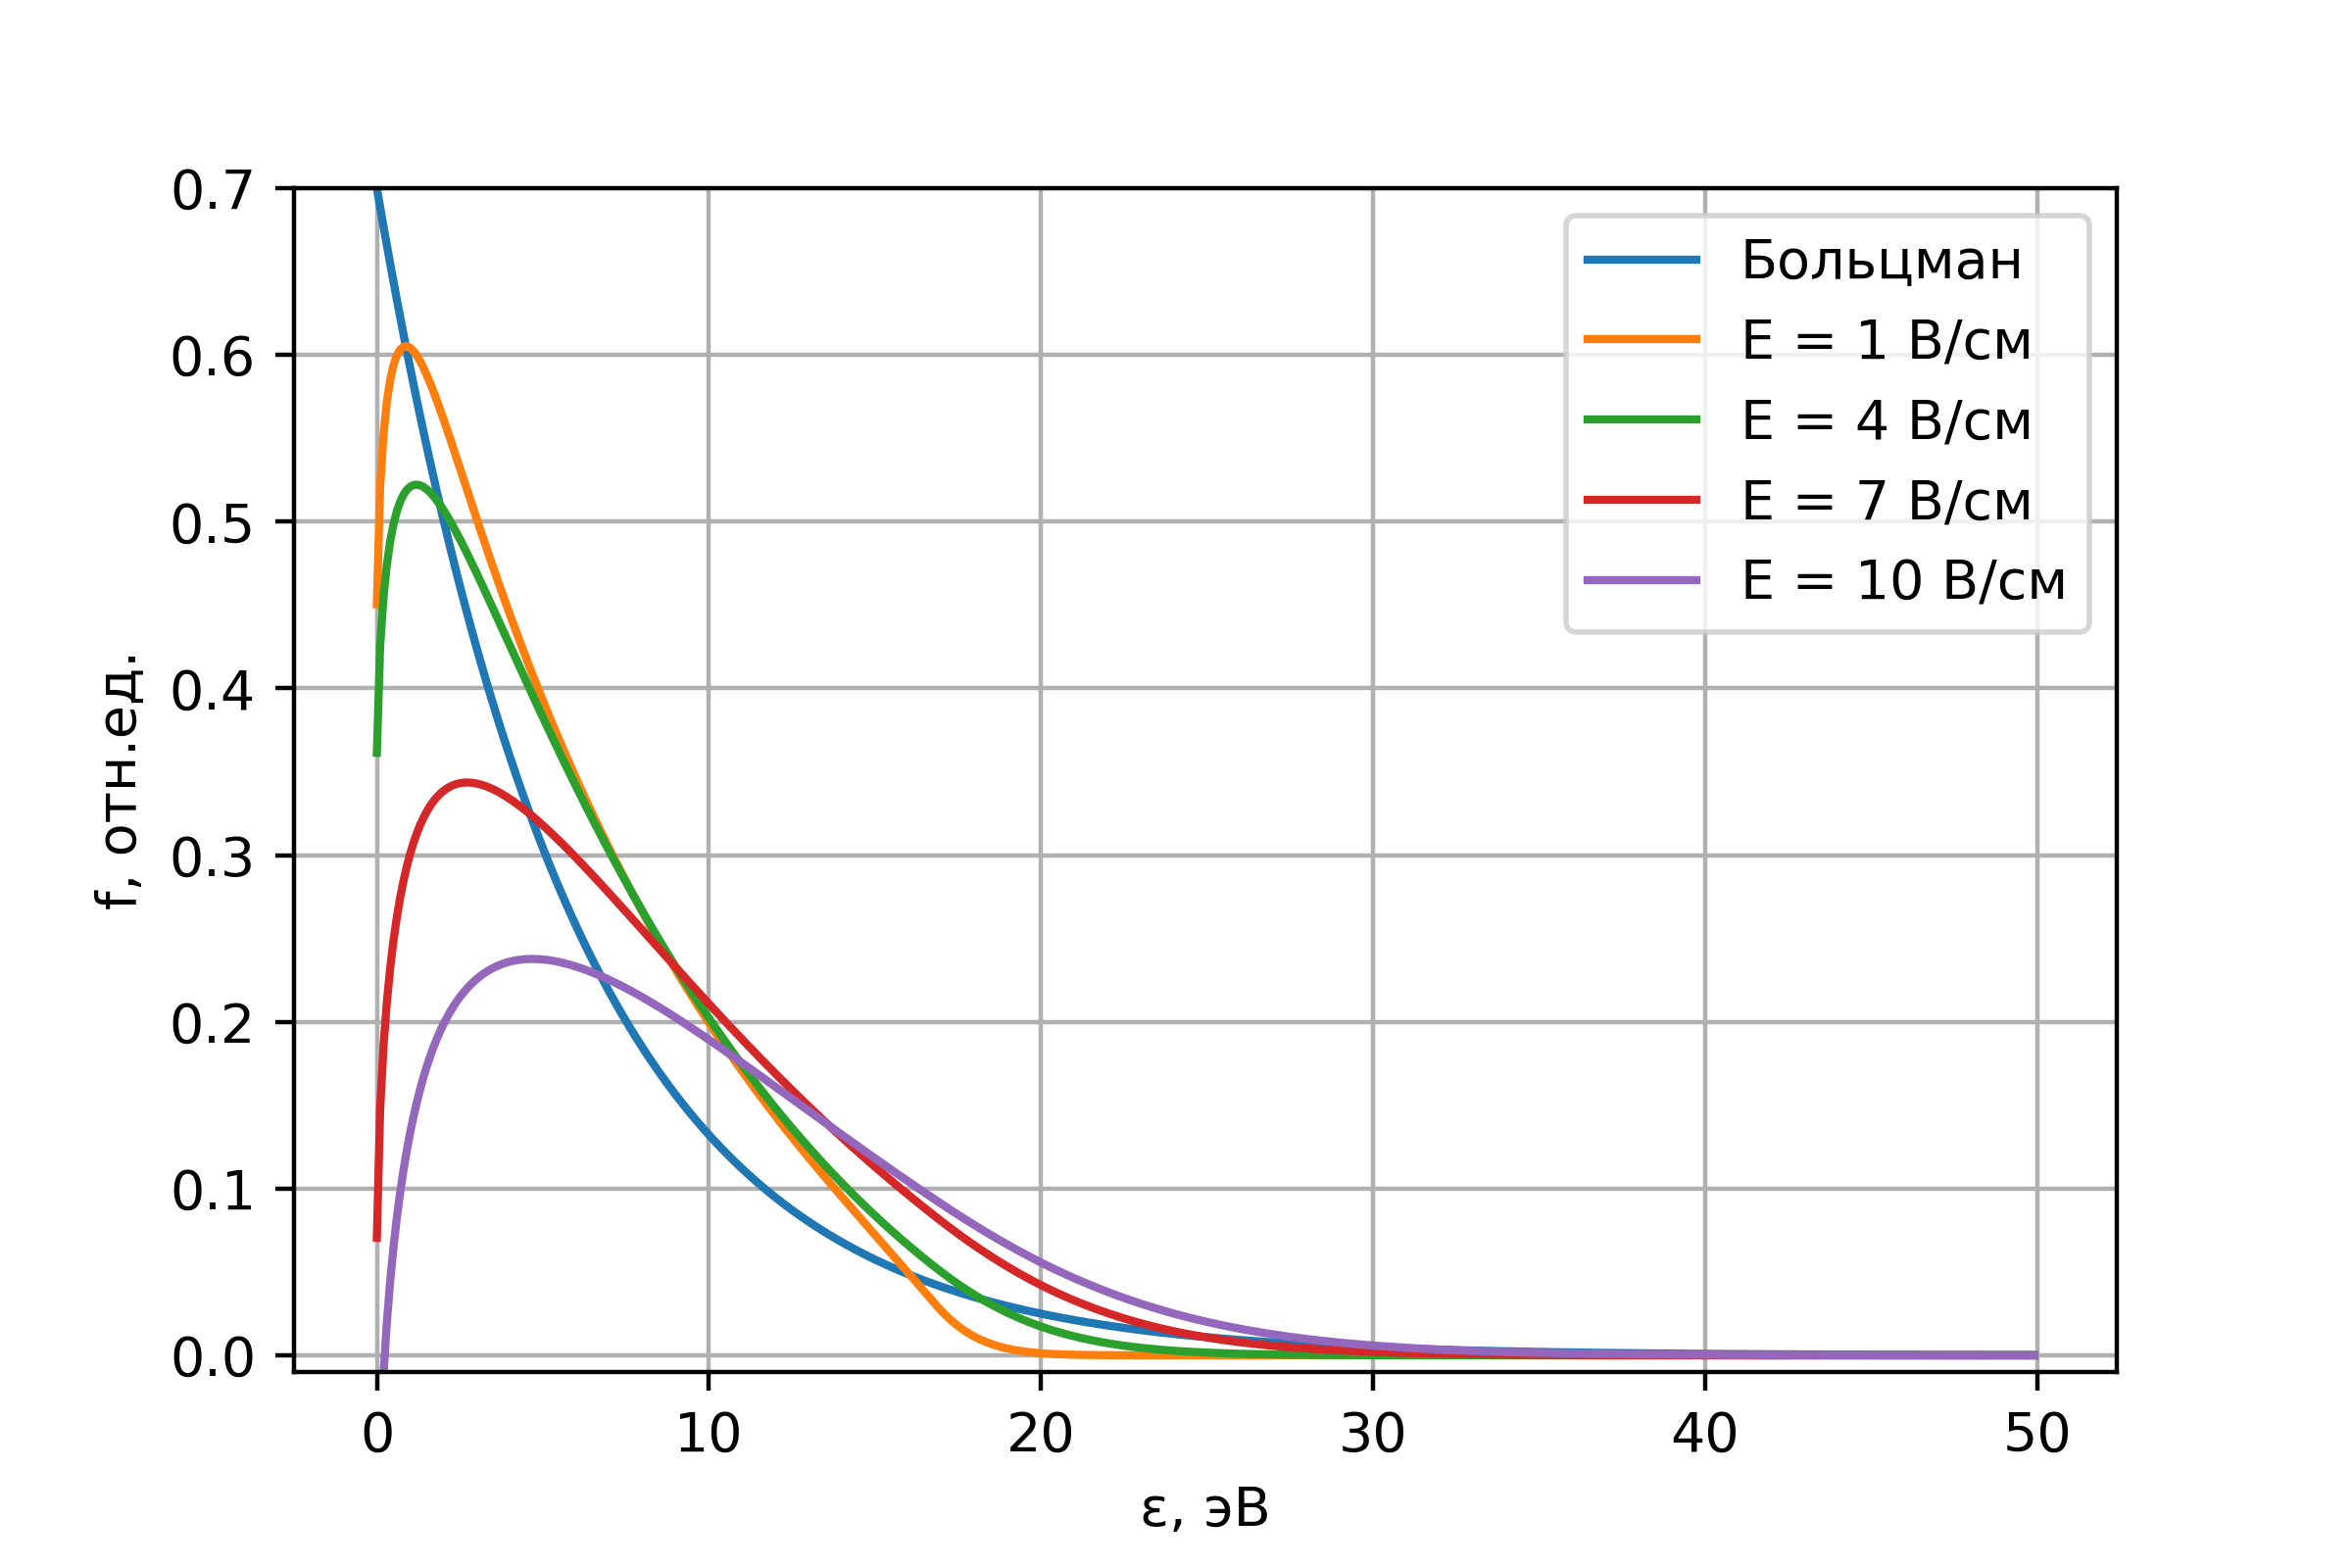
\includegraphics[width=15cm]{figures/fre_full}
  \caption{Зависимость расчетной функции распределения электронов от энергии и осевого электрического поля $E$,
  заданного параметрически для некоторых его значений; также нанесено распределение Больцмана, которое использовалось в качестве
  начального условия (\ref{eq:start_condition}).}
  \label{fig:fre_full}
\end{figure}
\begin{equation*}
    \sigma_t(\epsilon) = \begin{cases}
    \big{[}
        2.56 + 0.57 \cdot \ln
        \big{(}
            0.02 + {\epsilon \over 5.5 + \epsilon^2 } + {0.15 \cdot \epsilon^2 \over 12 + \epsilon + 3 \cdot 10^{-5} \cdot \epsilon^4}
        \big{)}
    \big{]} \cdot 10^{-16}, \epsilon > 0 \\
    \big{[}2.56 + 0.57 \cdot \ln(0.02)\big{]} \cdot 10^{-16}, \epsilon \le 0
    \end{cases}cm^2,
\end{equation}
\begin{equation*}
    \sigma_{16.62}(\epsilon) = \begin{cases}
    {2.742 \cdot 10^{-14} \over \epsilon^3} \cdot \sqrt{\epsilon - 16.6 \over \epsilon}, \epsilon > 16.62 \\
    0, \epsilon \le 16.62
    \end{cases}cm^2,
\end{equation}
\begin{equation*}
    \sigma_{16.67}(\epsilon) = \begin{cases}
    {5.01 \cdot 10^{-17} \over \epsilon} \cdot \sqrt{\epsilon - 16.67 \over \epsilon}, \epsilon > 16.67 \\
    0, \epsilon \le 16.67
    \end{cases}cm^2,
\end{equation}
\begin{equation*}
    \sigma_{16.72}(\epsilon) = \begin{cases}
    {5.941 \cdot 10^{-15} \over \epsilon^3} \cdot \sqrt{\epsilon - 16.7 \over \epsilon}, \epsilon > 16.72 \\
    0, \epsilon \le 16.72
    \end{cases}cm^2,
\end{equation}
\begin{equation*}
    \sigma_{16.85}(\epsilon) = \begin{cases}
    6 \cdot 10^{-18} \cdot \ln\big{(}{\epsilon \over 16.8}\big{)} + 5.7 \cdot 10^{-18} \sqrt{\epsilon - 16.8 \over \epsilon}, \epsilon > 16.85 \\
    0, \epsilon \le 16.85
    \end{cases}cm^2,
\end{equation}
\begin{figure}[t]
    \begin{center}
         \subfloat[\label{sub:log_fre_start}]{
           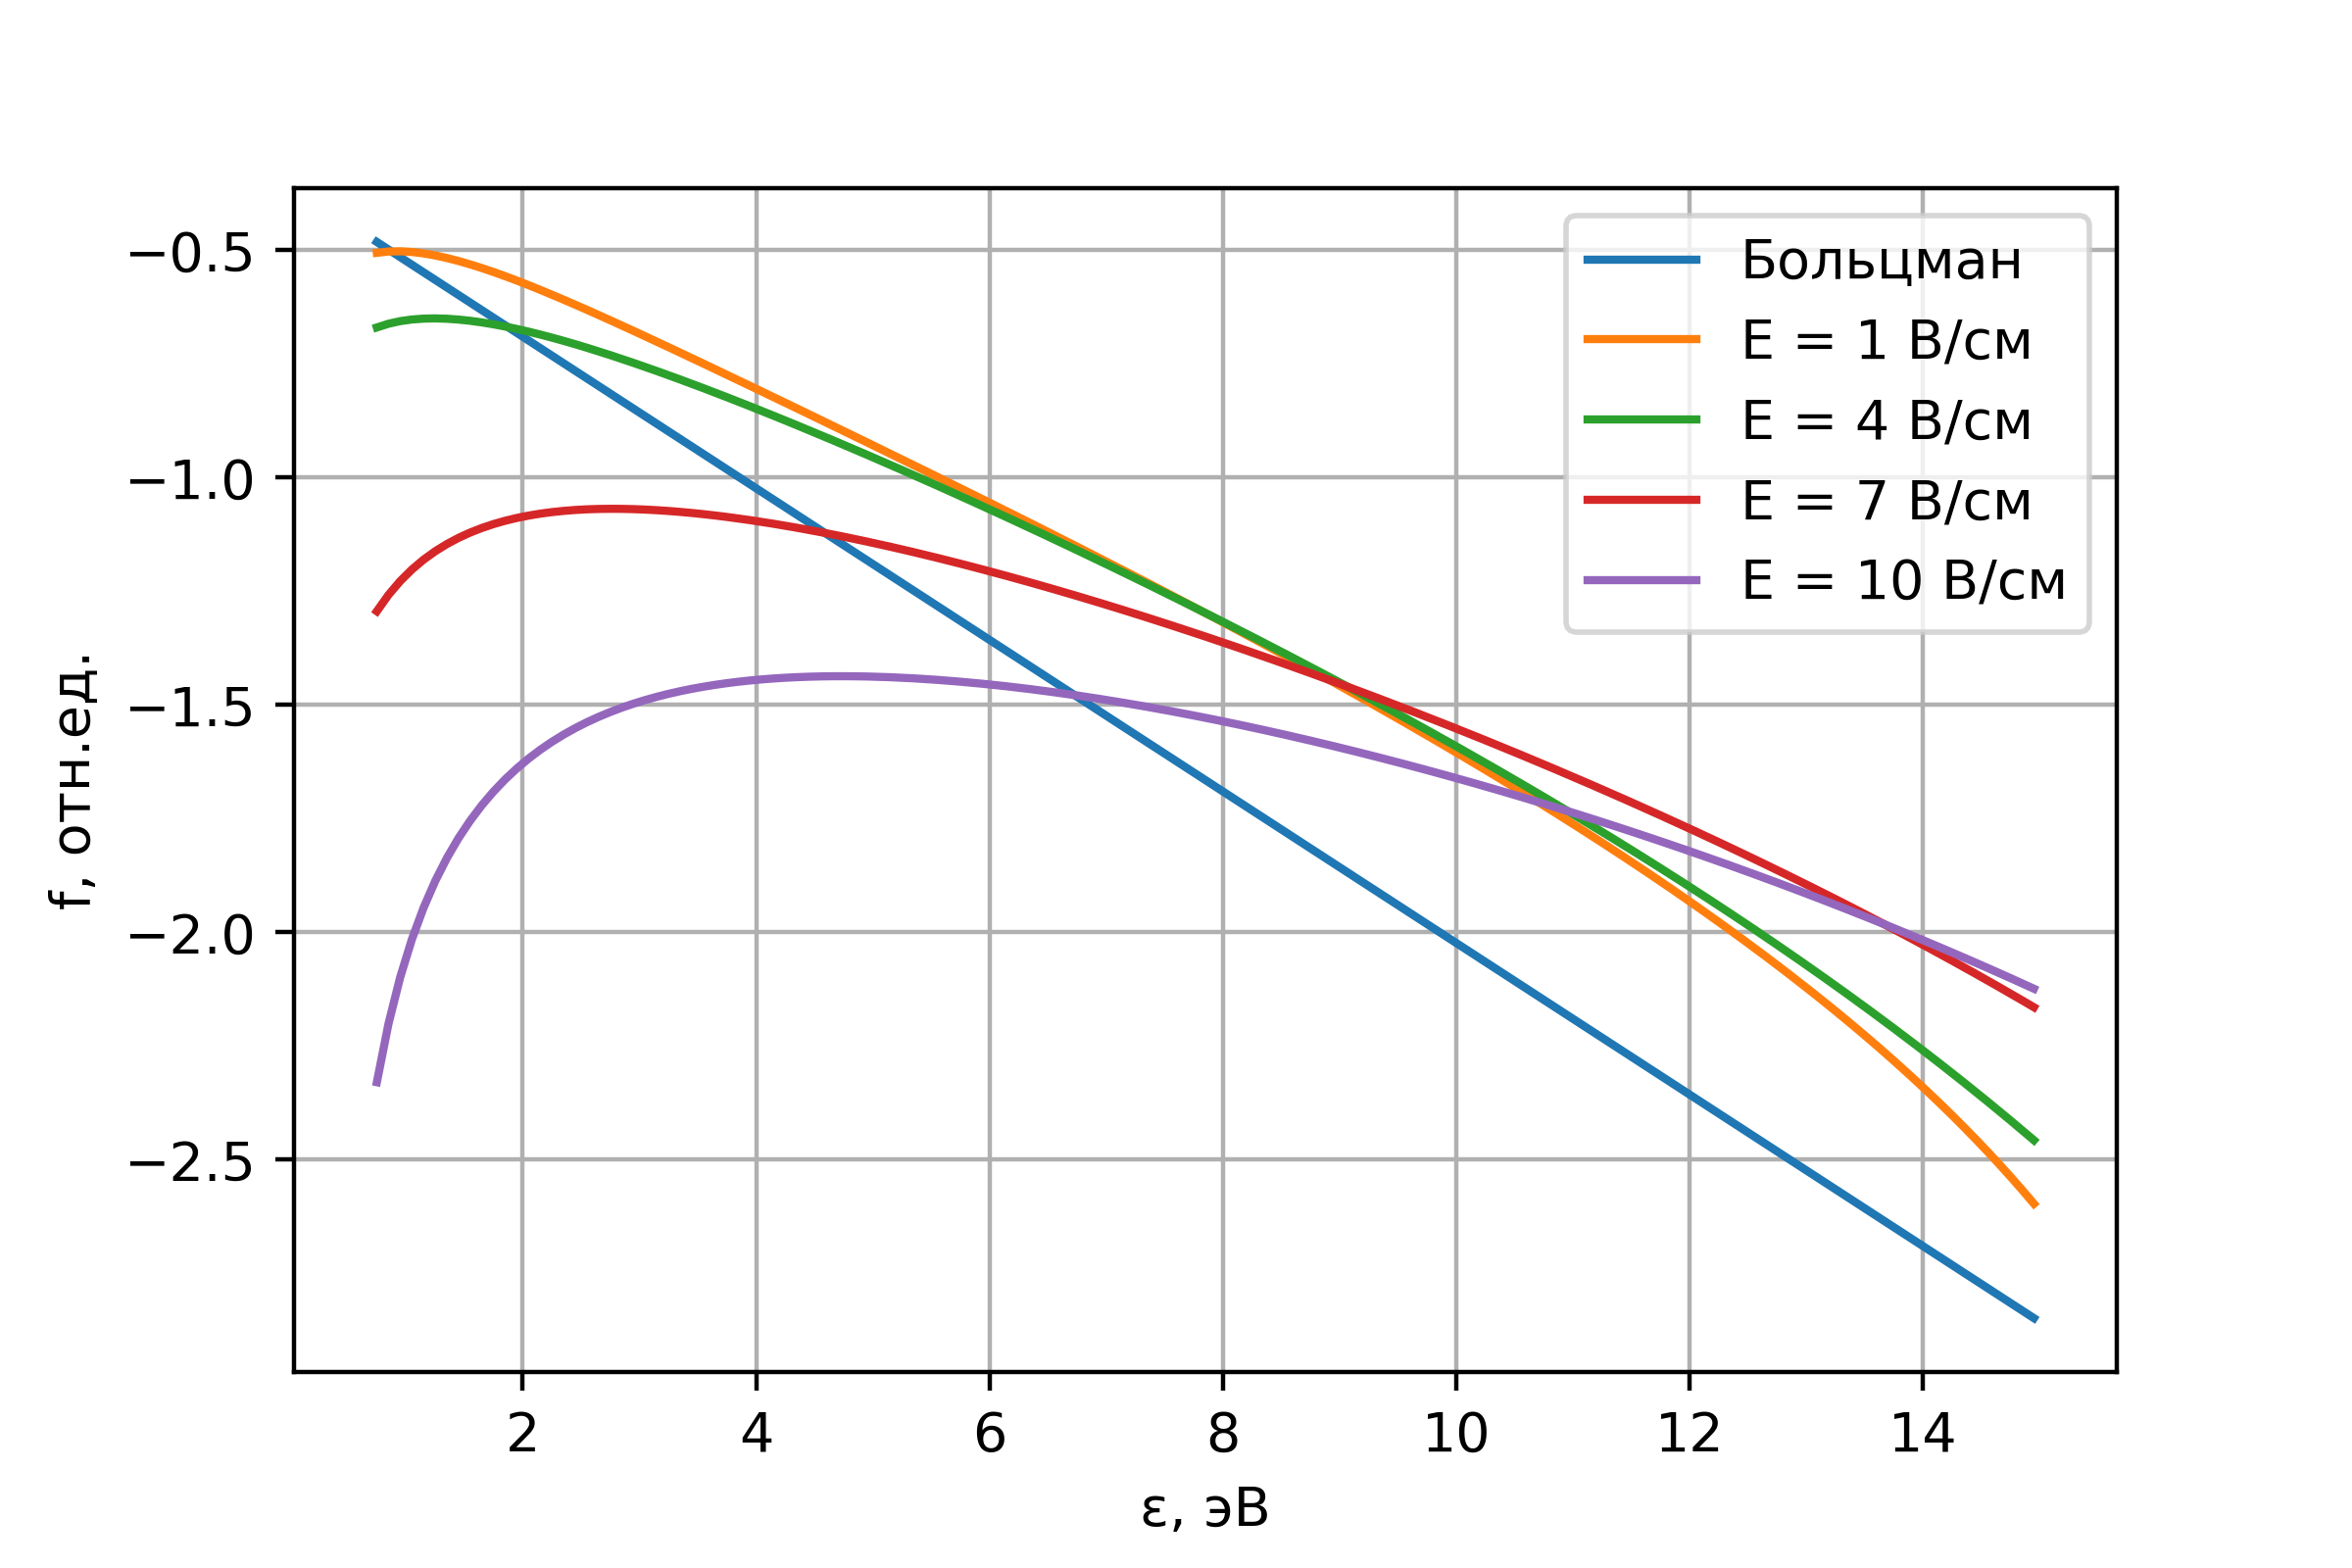
\includegraphics[width=0.49\textwidth]{figures/log_fre_start}
         }
         \subfloat[\label{sub:log_fre_tail}]{
           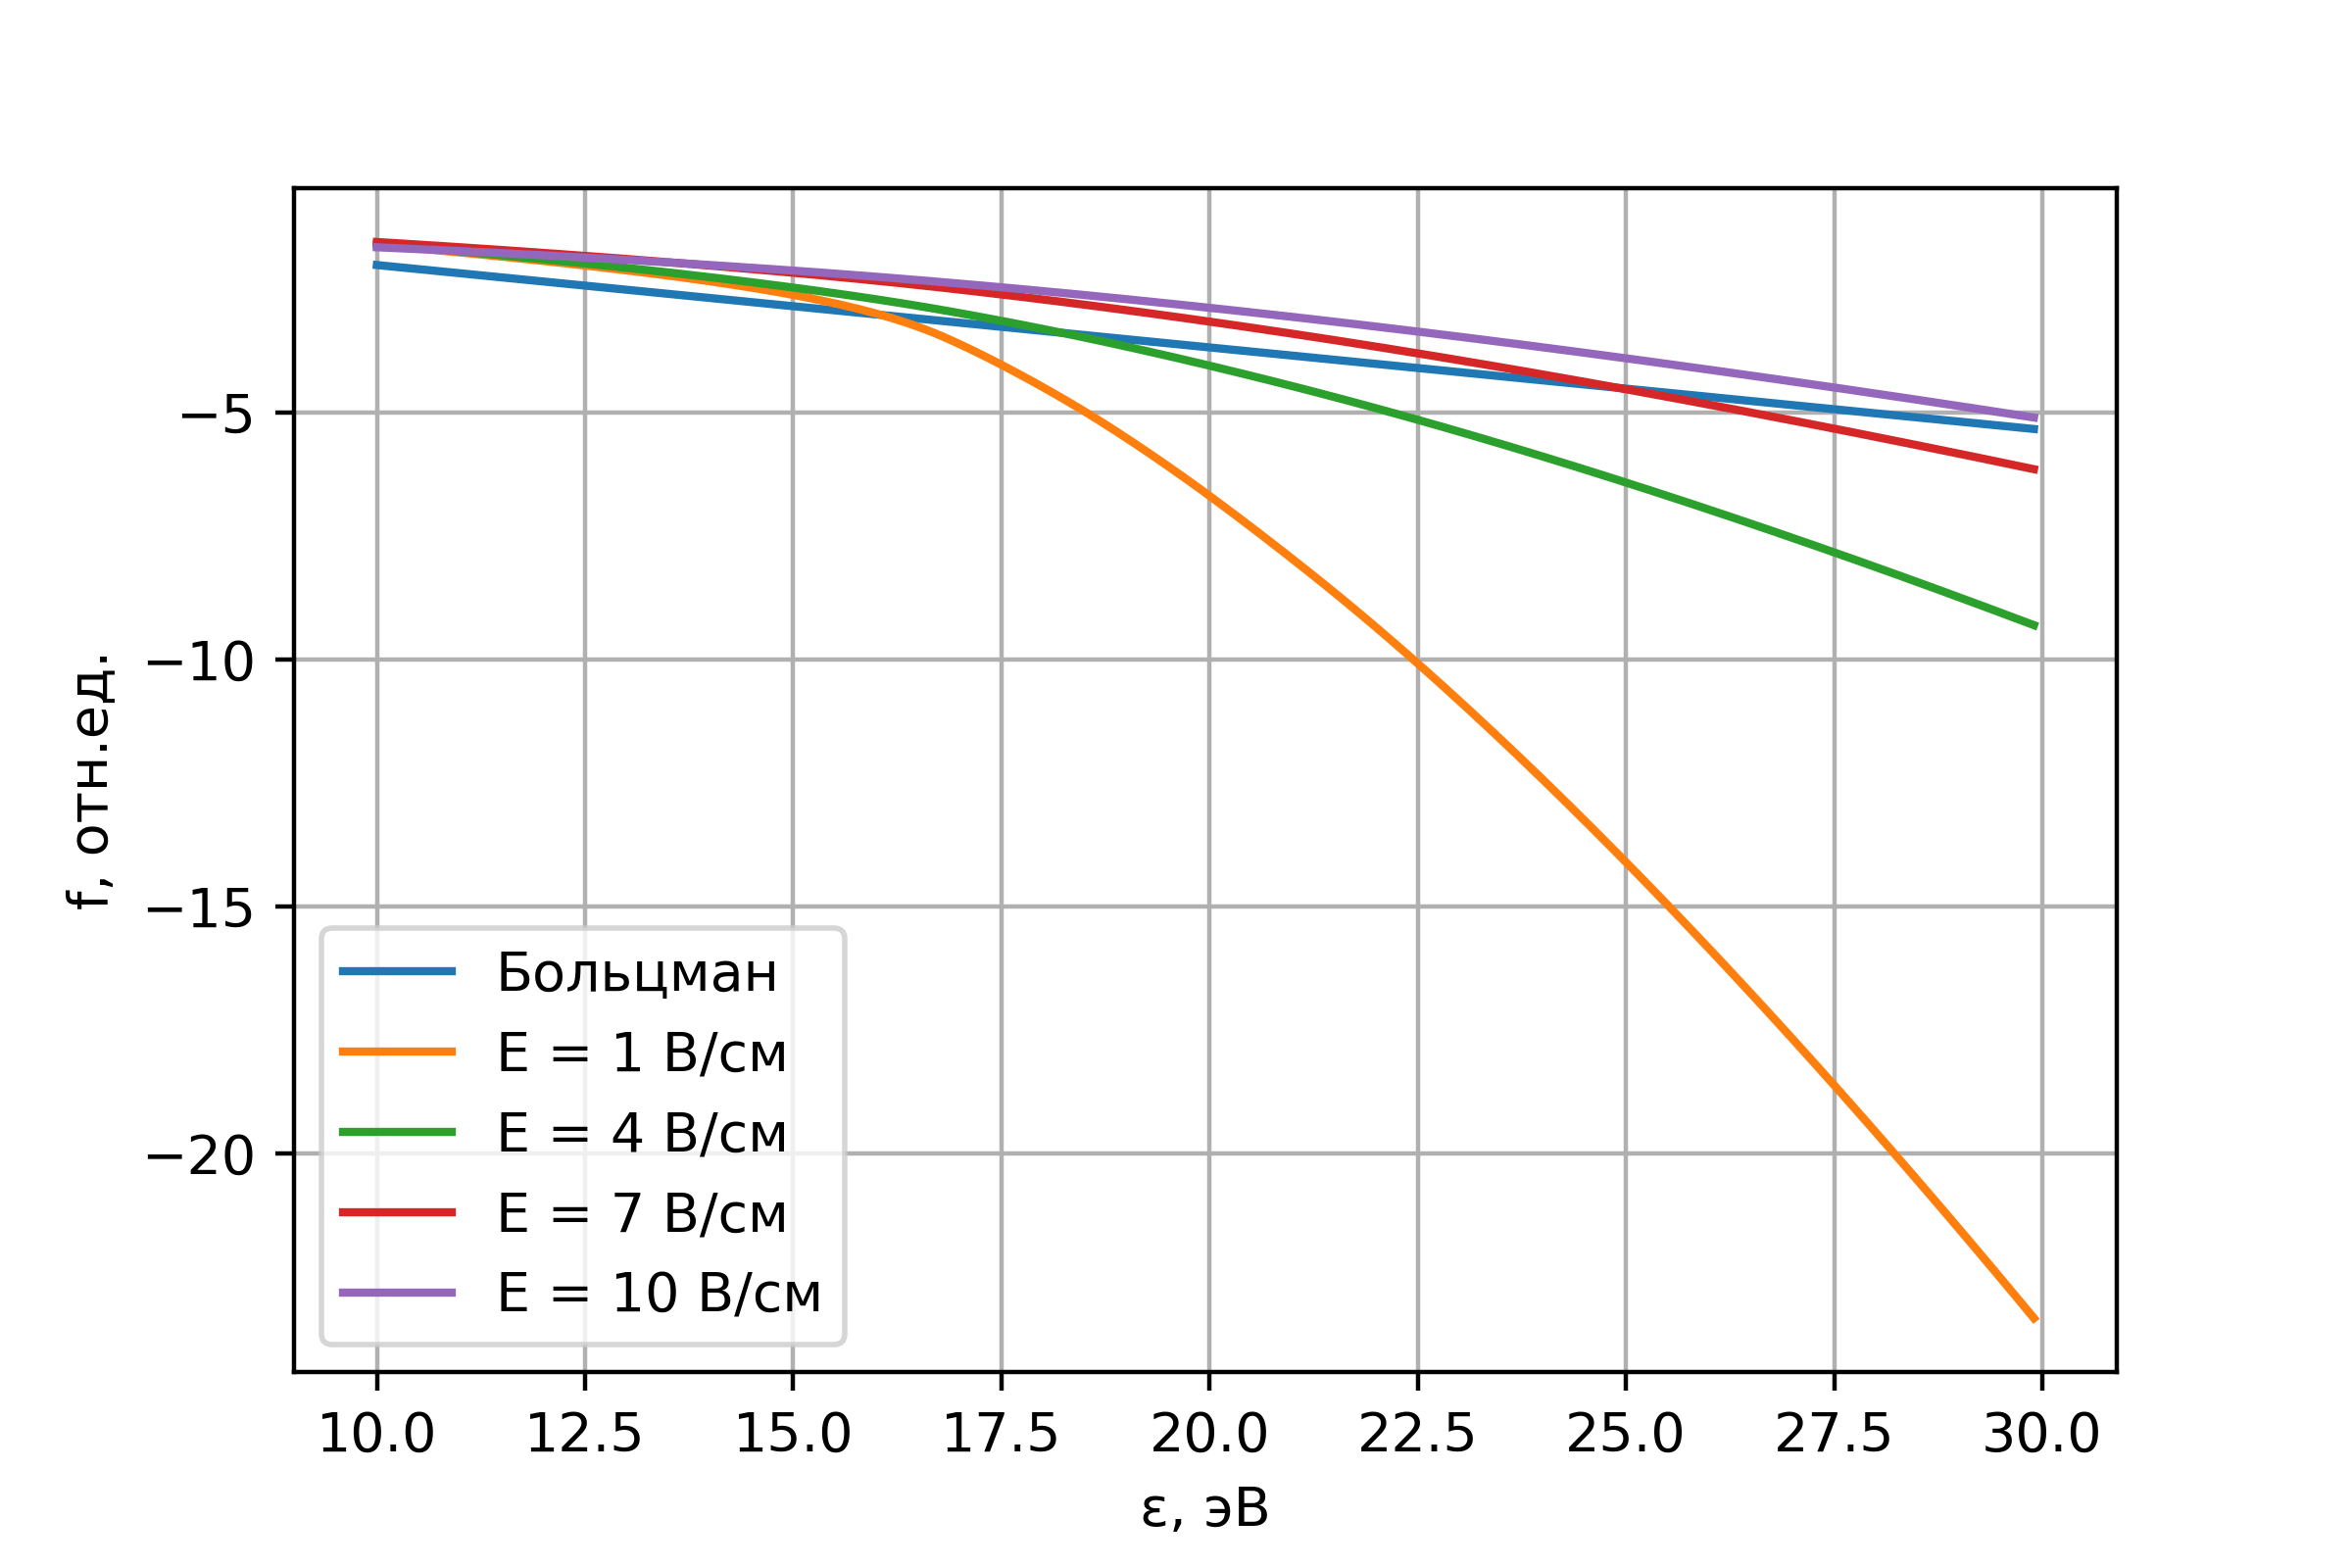
\includegraphics[width=0.49\textwidth]{figures/log_fre_tail}
         }
         \caption{Зависимость расчетной функции распределения электронов от энергии и осевого электрического поля,
                  заданного параметрически для некоторых значений, в логарифмическом масштабе:
                  \pt(а) в диапазоне \math{1 \le \epsilon \le 15 }$~эВ, \pt(б) в диапазоне \math{10 \le \epsilon \le 30 }$~эВ;
                  также нанесено распределение Больцмана, которое использовалось в качестве начального условия (\ref{eq:start_condition}).
         }
         \label{fig:log_fre}
    \end{center}
\end{figure}
\begin{equation*}
    \sigma_{18.38}(\epsilon) = \begin{cases}
    {2.024 \cdot 10^{-17} \over \epsilon + 11} \cdot \sqrt{\epsilon - 18.38 \over \epsilon}, \epsilon > 18.38 \\
    0, \epsilon \le 18.38
    \end{cases}cm^2,
\end{equation}
\begin{equation*}
    \sigma_{18.6}(\epsilon) = \begin{cases}
    {1.44 \cdot 10^{-16} + 1.4 \cdot 10^{-18} \cdot \epsilon \over \epsilon + 50} \cdot \sqrt{\epsilon - 18.6 \over \epsilon}, \epsilon > 18.6 \\
    0, \epsilon \le 18.6
    \end{cases}cm^2,
\end{equation}
\begin{equation*}
    \sigma_{18.71}(\epsilon) = \begin{cases}
    {3.461 \cdot 10^{-15} + 1.565 \cdot 10^{-16} \cdot \epsilon + 1.5 \cdot 10^{-18} \cdot \epsilon^2 \over (\epsilon + 37.4)(\epsilon + 27)} \cdot \sqrt{\epsilon - 18.7 \over \epsilon}, \epsilon > 18.71 \\
    0, \epsilon \le 18.71
    \end{cases}cm^2,
\end{equation}
\begin{equation*}
    \sigma_{18.97}(\epsilon) = \begin{cases}
    {7.6 \cdot 10^{-17} \over \epsilon} \cdot \ln\big{(}{\epsilon \over 18.97}\big{)}, \epsilon > 18.97 \\
    0, \epsilon \le 18.97
    \end{cases}cm^2,
\end{equation}
\begin{equation*}
    \sigma_{19.7}(\epsilon) = \begin{cases}
    1.8 \cdot 10^{-18} \cdot \sqrt{\epsilon - 19.7 \over \epsilon}, \epsilon > 19.7 \\
    0, \epsilon \le 19.7
    \end{cases}cm^2,
\end{equation}
\begin{equation*}
    \sigma_{20.0}(\epsilon) = \begin{cases}
    1.5 \cdot 10^{-18} \cdot \sqrt{\epsilon - 20.0 \over \epsilon}, \epsilon > 20.0 \\
    0, \epsilon \le 20.0
    \end{cases}cm^2,
\end{equation}
\begin{equation*}
    \sigma_{ion}(\epsilon) = \begin{cases}
    2.5 \cdot 10^{-17} \cdot {\epsilon - 21.5 \over 21.5}, \epsilon > 21.5 \\
    0, \epsilon \le 21.5
    \end{cases}cm^2.
\end{equation}

Используя данные аппроксимации сечений, разностную схему, начальные и граничные условия (\ref{eq:razh_scheme}~--~\ref{eq:start_condition}),
итерационные шаги \math{\Delta \epsilon = 0.1}$~эВ и \math{\Delta t \sqrt{2 \over m} = 0.0002 }$~с~\math{\cdot}$~г^{\math{-{1 \over 2}}}$,
а также параметрически задавая осевое электрическое поле в диапазоне \math{1 \le E_z \le 10}$~эВ с шагом \math{\Delta E_z = 0.1}$~эВ,
рассчитаем ФРЭЭ. С графическим представлением некоторых результатов можно ознакомиться на рисунке~\ref{fig:fre_full}.

Интенсивность свечения плазмы определенной длины волны формируется поведением ФРЭЭ при энергиях больше пороговой (до бесконечности),
которая имеет значение соответственно переходу для данной длины волны. Поэтому особый интерес в данной работе представляет
хвостовая часть полученной функции распределения электронов: в основном пороговая энергия для энергетических переходов неона больше
16~эВ. В обычном масштабе обнаружить на глаз поведение хвостовой части ФРЭЭ представляется невозможным (см.~рисунок~\ref{fig:fre_full}):
хвостовая часть распределения Больцмана, как и остальных посчитанных распределений, сливаются между собой. Поэтому удобнее
всего перейти к логарифмическому масштабу ФРЭЭ (см.~рисунок~\ref{fig:log_fre}\subref{sub:log_fre_tail}).

\section{Связь относительного изменения электронной температуры с отношениями интенсивностей спектральных линий}
\label{sec:link_ratio_and_TE}
Приведенные ранее рассуждения рассчета ФРЭЭ справедливы не только для невозмущенного пылевыми частицами положительного
столба газового разряда постоянного тока, но и для его возмущенного состояния. При добавлении пылевого облака в
разряд, концентрация частиц которого намного меньше концентрации электронов $n_d~\ll~n_e$, электроны по большей мере также
взаимодействуют с электронами: столкновениями с нейтралами можно пренебречь по аналогии со столкновениями с атомами.
На основе этих рассуждений можно сделать важный промежуточный вывод, что пылевые частицы не влияют определяющим образом
на ФРЭЭ, а лишь изменяют параметры разряда, от которых зависит ФРЭЭ.

Для невозмущенного положительного столба газового разряда постоянного тока функция распределения электронов по
энергиям принимает двухтемпературный вид для энергетических интервалов $1 \le \epsilon \le 16$~эВ и
$17 \le \epsilon \le 30$~эВ~\cite{Zobnin2018}, что и наблюдается в полученных расчетах (см.~рисунок~\ref{fig:log_fre}).
Данное распределение объясняется тем, что электроны при достаточно больших энергиях начинают неупруго взаимодействовать
между собой, что и дает вклад в электронную температуру. Поскольку электроны высвечивают лишь в ходе неупругих взаимодействий, то
спектральные данные не содержат информацию о ФРЭЭ до $16.4$~эВ (энергия первого возбужденного состояния неона), а лишь
несут информацию о хвостовой части ФРЭЭ (см.~рисунок~\ref{fig:log_fre}\subref{sub:log_fre_tail}).
Запишем распределение хвостовой части ФРЭЭ в больцмановской аналогии:
\begin{equation}
    f_{tail}(\epsilon) = e^{-{\epsilon \over T_e}} \Rightarrow ln(f_{tail}) = - {\epsilon \over T_e}.
    \label{eq:tail}
\end{equation}

В рамках одного и того же переходного процесса справедливы следующие рассуждения: интенсивность
спектральной линии пропорциональна заселенности возбужденного уровня данного перехода, которая в свою очередь
пропорциональна скоростному коэффициенту заселения прямым электронным ударом с основного состояния:
заселение с метастабильных состояний и переходы электронов с более высоких уровней модель не рассматривает~(см.~раздел~\ref{sec:kinetika}), т.е.:
\begin{equation}
I_{j,i}(T_e) \sim N^*_{j}(T_e) \sim X_{0,j}(T_e).  % \sim  \int_{E_{th}}^{\infty} \sigma(\epsilon)f_{tail}(\epsilon)\sqrt{\epsilon}d\epsilon
\label{eq:sim_Te}
\end{equation}

Используя выражения (\ref{eq:X_0j}) и (\ref{eq:sim_Te}) для двух различных конфигураций газового разряда для выбранной
спектральной линии в рамках одного переходного процесса $j$, имеем:
\begin{equation}
{{I_2} \over {I_1}}= {{\int_{E_j}^{\infty} \sigma_{E_j}(\epsilon)f_{2}(\epsilon)\epsilon d\epsilon} \over
{\int_{E_{j}}^{\infty} \sigma_{E_j}(\epsilon)f_{1}(\epsilon)\epsilon d\epsilon}},
\label{eq:intensities_ratio}
\end{equation}
где индексы 1 и 2 обозначают различные конфигурации самосогласованного газового разряда, т.е. при различных осевых
электрических полях. Следует отметить, что энергия возбужденного уровня $E_j$ влияет на значение отношения интенсивностей,
что и наблюдается в работах \cite{Pikalev2018}, \cite{Kostenko} и \cite{Samsonov1999}.

Таким образом, выполнив перебор всех расчетных ФРЭЭ для различных осевых электрических полей, можно понять по экспериментальным
отношениям интенсивностей спектральных линий и (\ref{eq:intensities_ratio}), какая из ФРЭЭ описывает новую конфигурацию
газового разряда. Затем по хвостовой части ФРЭЭ из (\ref{eq:tail}) несложно вычислить и электронную температуру хвостовой части:

\begin{equation}
    T_{e,2} = {{ln(f_{tail,1}(\epsilon)) \over ln(f_{tail,2}(\epsilon))} T_{e,1}} \Big{\rvert}_{\forall \epsilon: \epsilon \in tail} .
    \label{eq:Te_from_FRE}
\end{equation}